\documentclass[11pt, a4paper, titlepage]{article}
\usepackage[margin=3.5cm]{geometry}
\usepackage{graphicx}
\usepackage[table,xcdraw]{xcolor}
\usepackage{minted}
\usepackage{dirtree}
\usepackage[utf8]{inputenc}
\usepackage[english]{babel}
\usepackage[backend=bibtex]{biblatex}
\usepackage{appendix}
\addbibresource{biblio24.bib}

\begin{document}
\begin{titlepage}
	% Logo at the top within the margins
	\noindent
	
\includegraphics[width=0.15\paperwidth]{logo-mg.png} % Adjust the size as needed
	
	% Title and subtitle with left offset
	\vspace*{0.5\paperwidth} % Adjust the vertical space as needed
	\noindent\hspace*{0.15\paperwidth} % Offset from the left
	\begin{minipage}{\textwidth}
		
		\color[HTML]{0b5394}\Huge Magisim\\
		\color{black}\Large Open source resource center for simulations \\
	\end{minipage}
	
	\vfill % Push the authorship information to the bottom of the page
	\noindent
	\begin{minipage}{\textwidth}
		\normalsize % 12pt font size
		Jonas Cronholm \\
		\textbf{Gymnasiearbete 100 poäng} \\
		\textbf{Klass:} 21 TE \\
		\textit{Teknikprogrammet} \\
		\textbf{Läsåret:} 2023-2024 \\
		\textbf{Handledare:} Peter Eriksson
	\end{minipage}
\end{titlepage}

% Titlepage for arXiv - Needs style changes soon!
% 
%\begin{titlepage}
%	\title{
\includegraphics[width=0.35\textwidth]{magisim_logo256.png}\par\vspace{1cm}Magisim: Open source resource center for electromagnetic simulations \let\thefootnote\relax\footnotetext{Gymnasiearbete 100p}}
%	\author{Jonas Cronholm, Rasmus C. Ljung}
%	\maketitle
%\end{titlepage}
%
\newpage
\
\newpage

\begin{abstract}
	
	With serious competition in the modern market it is not trivial to create a product that can match the expectations of professional users and still appeal to hobby engineers, especially at a modest price point. The gap in capabilities between enterprise and open source simulation software is growing bigger due to lack of funding, which often results in limited research and development for free and open source projects. This growing disparity poses a significant challenge for developers aiming to balance advanced features with affordability. 
	
	Enterprise simulation software benefits from substantial financial backing, enabling teams to invest in cutting-edge research, continuous enhancements, and dedicated customer support. This translates to robust features, high accuracy, and comprehensive technical support, making them the preferred choice for intricate and mission-critical projects. However, the cost associated with these solutions can be prohibitive for smaller businesses and individual hobbyists. This gap is further exacerbated by the intricate nature of simulation software. Meeting the needs of professionals frequently involves complex algorithms, intricate modeling, and high-performance computing. Striving to offer similar capabilities within a modest price range for hobbyists can be daunting, as the associated costs can quickly spiral upwards.
	
	Addressing this challenge, Magisim, an open-source project developed using modern tools such as machine learning technology, is introduced as a versatile solution. Designed primarily as an educational tool, Magisim allows for the integration of a wide range of simulation algorithms, and the programming of data flow using a node graph interface. This approach not only democratizes the learning and application of complex simulations but also bridges the gap in performance between high-cost enterprise solutions and open-source software. Consequently, Magisim serves as a testament to the potential of open-source development in narrowing the divide in technological capabilities, fostering an environment where both professionals and hobbyists can explore, learn, and contribute to the evolving field of simulation and data analysis.
	
	
	%This paper presents a proof-of-concept software project that aims to illustrate the potential of open source magnetic field simulations utilizing parallelized computing techniques on consumer-grade hardware. Magnetic field simulations hold immense significance across scientific, engineering, and technological domains, yet their resource-intensive nature often limits accessibility, particularly in the context of proprietary software and high-cost hardware. By conducting a thorough analysis of existing open source simulation tools, parallel computing frameworks, and optimization strategies, we lay the groundwork for a proof-of-concept that showcases the potential of democratizing magnetic field simulations. This paper provides an in-depth exposition of the technical underpinnings involved in parallelization implementation, optimization techniques, and comprehensive performance evaluations. Through our preliminary experimentation, we offer empirical evidence of substantial reductions in simulation runtime while maintaining accuracy levels comparable to established proprietary solutions.
	
	%Moreover, the paper acknowledges and addresses the inherent challenges intrinsic to parallel programming, hardware limitations, and scalability concerns when deploying simulations on consumer-grade hardware. By providing practical insights and strategic recommendations, we outline potential avenues to navigate these challenges and attain optimal performance across varying hardware configurations.
	\begin{flushleft}
		{\small {\bf Keywords:} Computational electromagnetics, CEM, MoM, FEM, parallelization, simulator, CUDA, gradio, Data Analysis, Visualization}
	\end{flushleft}
	\hspace*{\textheight}
	\begin{flushright}
		\it{"An idiot admires complexity. A genius admires simplicity." - Terry A. Davis}
	\end{flushright}
	
	
\end{abstract}
\refstepcounter{page}
\setcounter{page}{2}
\tableofcontents
\newpage
%\twocolumn[]
\section{Introduction}
\subsection{Background}
The field of radio engineering, particularly within the amateur radio sphere, necessitates a deep understanding of electromagnetic (EM) theory and its practical applications. Traditionally, this domain has been supported by a variety of simulation tools, aiming to provide insights into the complex interactions of electromagnetic fields with their surrounding environments. However, a significant challenge has emerged from the existing landscape of these simulation tools, marked by their prohibitive cost and steep learning curves. This divide presents a substantial barrier to entry for amateur radio enthusiasts and learners, who often seek both affordability and simplicity in educational resources. 

\subsection{Problem}
Historically, professional-grade simulation software in electromagnetics has been tailored to meet the demanding needs of industry experts, incorporating advanced features and comprehensive simulation capabilities. While powerful, these tools come at a price point that is often beyond the reach of hobbyists and educational users. Concurrently, the free or low-cost alternatives available in the market tend to compromise either on the width of features or on user accessibility. The complexity of these tools, coupled with often inadequate documentation, further exacerbates the challenge for those new to the field, impeding practical, hands-on learning.

This gap in the market led to the conceptualization of Magisim, initially envisioned as a user-friendly and cost-effective simulator specifically for electromagnetics. Targeted towards the amateur radio community, the primary goal was to demystify EM theory through interactive simulations, making it more approachable for non-professionals. However, as the project progressed, we realized the broader potential for the underlying technology. The modularity of our initial design, made the software applicable in more fields related to simulations or data analysis. This steered the development of Magisim towards becoming a more versatile platform, transcending its original scope.

In the last few years, machine learning has become one of the most important tools in many fields, including software development. This project also aims at benchmarking the code production quality, efficacy and finding new ways of accelerating the development process of software using Large Language Models (LLMs) as a central tool.

\newpage

\subsection{Introduction to Computational Electromagnetics}
Computational electromagnetics (CEM) is a field of study that employs numerical methods to solve problems that involve electromagnetic interactions. These computational methods are essential for designing, analyzing, and optimizing electronic and optical devices, such as antennas, radar, waveguides, and optical systems.

A key technique in CEM is the Finite-Difference Time-Domain (FDTD) method, which simulates electromagnetic field behavior by solving Maxwell's equations across a discretized spatial and temporal grid. This method is prized for its ability to model complex interactions in various materials and structures accurately. FDTD is particularly useful in fields such as antenna design, optical device analysis, and electromagnetic compatibility testing. It allows for a detailed examination of how electromagnetic waves propagate and interact with their environment, making it an essential tool for both researchers and engineers. In educational settings, tools like Magisim utilize FDTD to help students and hobbyists understand and visualize electromagnetic phenomena in a straightforward and accessible manner.


\subsection{Related Work}
\subsubsection{Proprietary Software}
Many solutions exist for simulating electromagnetic systems, particularly in the realm of proprietary software that offers advanced capabilities but often at a cost that is prohibitive for amateurs. Tools like Ansys HFSS, Altair FEKO, and XFdtd are common in this field, each providing specialized features tailored to complex and precise electromagnetic simulation needs.

\textbf{Ansys HFSS (high-frequency structure simulator)} excels in using the Finite Element Method for detailed electromagnetic field simulations, ideal for high-frequency electronics and antenna design. \textbf{Altair FEldberechnung für Körper mit beliebiger Oberfläche (FEKO)} offers a broad range of computational methods, making it versatile for applications across electromagnetic compatibility and antenna design, amongst others. \textbf{XFdtd} utilizes the Finite-Difference Time-Domain method, suitable for transient electromagnetic simulations and interactions, such as EMC testing and bioelectromagnetic analyses.

Despite their robust features and extensive applications, these tools are often not accessible to the common amateur due to their high cost and the complex technical expertise required. This creates a significant barrier for hobbyists and smaller enterprises who might not have the resources or need for such advanced functionalities.
\newpage

\subsubsection{Open Source Projects}
In the field of electromagnetic simulations, the openEMS tool, described by Liebig et al. (2012)\cite{liebig12}, stands out as a noteworthy open-source platform leveraging the Finite-Difference Time-Domain (FDTD) method. This tool, freely available to the public, supports various simulation needs, particularly for high-frequency electromagnetic applications. The openEMS platform uses an equivalent-circuit (EC) FDTD method, which simplifies the implementation of material dispersion, thus enhancing the simulation of complex electromagnetic environments. Although openEMS is a powerful tool, its depth and the required scripting for setup and control can be daunting for amateurs and new users.

In his PhD thesis, Novel architectures for brain-inspired photonic computers. Ghent University (2020)\cite{laporte20}, Floris Laporte employs a custom Finite-Difference Time-Domain (FDTD) simulator to analyze photonic structures that mimic neural processes for neuromorphic computing applications. Laporte's work focuses on the simulation aspect, using this method to delve into the dynamic behaviors of photonic cavities and their potential as elements in brain-inspired computing architectures. In developing our simulator, Magisim, we have integrated Laporte's FDTD code as a core component.


\subsection{Scope}


% What would be the scope?
% We set design rules for extensions in order to ease development
% We initially set our scope to be a CUDA-accellerated FDTD simulator,
% but realised that designing such software in the short time frame would
% be infeasible. we instead focused our efforts on making the software as
% modular as possible such as to allow future expansion.

Initially, we aimed to develop a CUDA-accelerated Finite-Difference Time-Domain (FDTD) simulator that could leverage the computational power of modern GPUs to enhance simulation speed significantly.
However, during the early stages of development, it became apparent that designing and implementing a fully CUDA-accelerated simulator within the project's limited timeframe was infeasible.
\begin{itemize}
	\item \textbf{Technical Complexity:} The integration of CUDA technology into the FDTD algorithm involves deep knowledge of parallel programming and optimization strategies that were beyond the immediate capabilities of the team.
	\item \textbf{Resource Constraints:} Limited access to necessary hardware and software resources to test and develop CUDA-accelerated features effectively.
	\item \textbf{Development Time:} The time required to learn, implement, and debug a CUDA-accelerated approach exceeded the project's scheduled timeline.
\end{itemize}

Given these challenges, the focus shifted towards enhancing modularity. This aimed at laying a robust foundation that could support future integrations of CUDA acceleration and other advanced features.
To facilitate development and ensure the software's long-term viability, a set of design rules for extensions was established. These guidelines serve multiple purposes:
\begin{itemize}
	\item \textbf{Ease of Development:} Simplifying the process for future contributors to develop and integrate new modules or features without extensive reworking of the existing codebase.
	\item \textbf{Consistency:} Maintaining a uniform architecture that supports the seamless functioning of diverse components developed by different contributors.
	\item \textbf{Expandability:} Allowing the simulator to evolve over time by accommodating new technologies and methodologies as they become viable.
\end{itemize}


\newpage

\newpage
\section{Method}
The initial phase of the project involved comprehensive planning using the Kanban system implemented through Atlassian Trello. This enabled efficient organization and prioritization of envisioned functionalities for the simulator and its interface. The systematic arrangement of tasks on the Kanban board facilitated a clear visualization of the project scope, ensuring effective integration of all functionalities. Subsequently, a Gantt chart was utilized to structure the project's timeline and responsibilities, allowing for a detailed outline of the time plan and division of labor. We also utilized machine learning models, such as Generative Pre-trained Transformer 4 (GPT-4)\cite{openai23} to further aid project planning, as well as for code completion.
\subsection{Project Structure}
The directory structure is as follows:
\dirtree{%
	.1 magisim.
	.2 docs.
	.3 <website sources for magisim.com>.
	.2 notebooks.
	.3 <development notes as well as this paper>.
	.2 resources.
	.3 <images, videos, gifs for the readme and website>.
	.2 src.
	.3 tests.
	.4 <development tests>.
	.3 ui.
	.4 extensionmgr.
	.4 extensions.
	.5 <user extensions get installed here>.
	.4 nodemgr.
	.4 projects.
	.5 <user saved projects are stored here>.
	.4 settingsmgr.
	.4 shapeloader.
	.4 shared.
	.5 <magisim resources such as type definitions>.
	.4 <scripts>.
}

\newpage


\subsection{User Interface}

Following the establishment of the project's framework and timeline, focus shifted to the user interface (UI) design for Magisim. Several UI development toolkits, including QT and GTK, were evaluated to determine the most suitable option based on modularity, integration ease, and development efficiency. Despite the admirable features of QT and GTK, challenges were encountered with their steep learning curves and complex integration processes, including licensing and cost constraints.

The search ultimately led to the selection of Gradio, a growing UI library distinguished by its modular design and streamlined development process. Gradio's capability for rapid prototyping and its intuitive user experience made it the preferred choice for the project, facilitating the swift iteration of UI components.
\begin{center}
	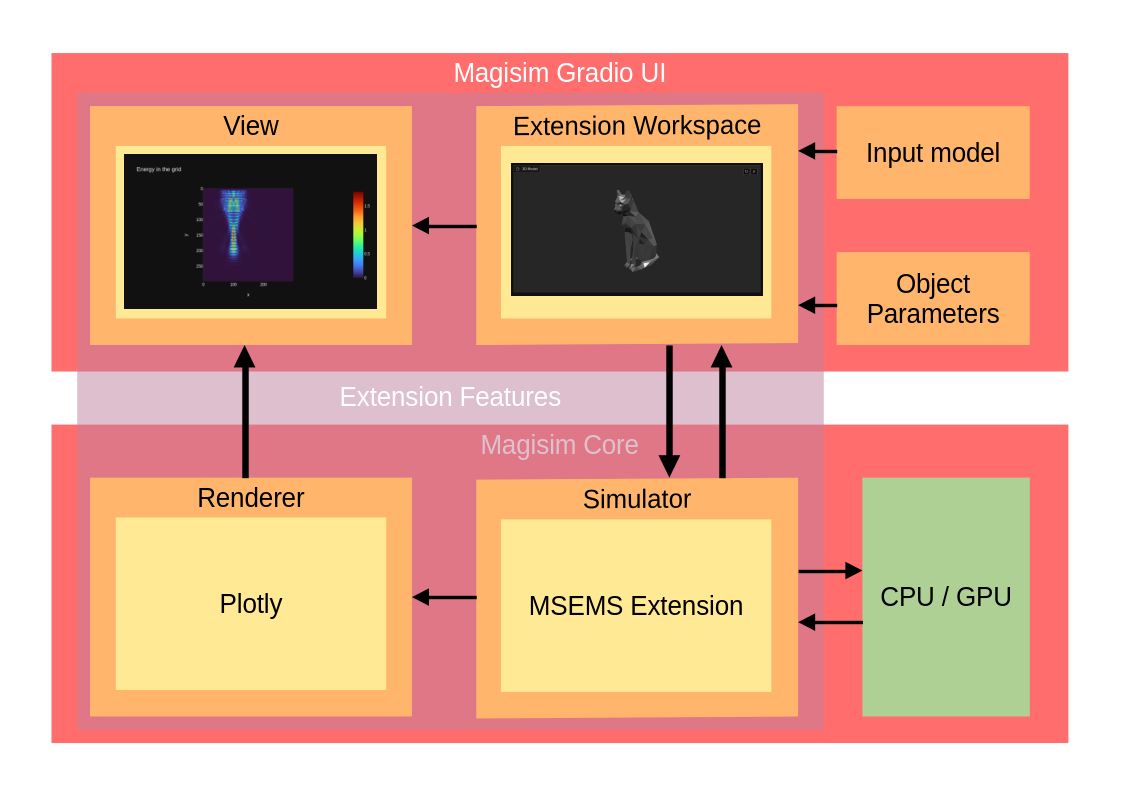
\includegraphics[width=0.8\textwidth]{softstruct.png}
\end{center}

Each extension describes its own user interface by using modules available in the Gradio package. This allows third parties to rapidly develop intuitive and efficient interfaces that integrate seamlessly with the core functionalities of Magisim. The use of Gradio's modules offers developers the flexibility to customize and extend the interface according to specific needs, developers may also create "custom components" allowing even more degrees of freedom.
\newpage
\subsection{Extension Model and Templates}

Aiming for high modularity, the project was structured so that every component was defined as an "Extension". This approach enabled the development of a unified system where all components adhered to a set of predefined rules, including a universal code structure. Such standardization allowed for the components to be loaded by a single function at startup, simplifying the development process and reducing program complexity.

\begin{minted}{python}
	# shared extension imports
	import gradio as gr
	from shared.builtin import Extension
	from shared.config import Config
	
	class ExtensionMeta:
	name: str = "name"
	uuid: str = "some-uuid-v4"
	authors: list = ["author"]
	version: str = "1.0.0"
	license: str = "license"
	description: str = """multiline description if needed"""

	class ExtensionType:
	types: list = [Extension.Simulator, Extension.Workspace]
	hasNodes: [(Extension,(list,list))] = [
	(Extension.Simulator, # define a simulator node
		(
			[ # inputs
				("some-input","some-type")
			],
			[ # outputs
				("some-output1","some-type"), 
				("some-output2","some-type")
			]
		)
	)]
	
	def load_workspace(app: gr.Blocks):
		with gr.Tab(ExtensionMeta.name, id=ExtensionMeta.uuid):
			gr.Markdown(ExtensionMeta.description)
			# Extension UI code

\end{minted}
\newpage

\subsection{Message Queue and Routing}

In defining component interaction and data handling, the initial consideration was to develop an in-house asynchronous communication layer. However, it was soon recognized that many solutions existed for such functionality. A message queue system in combination with a "Router" was eventually chosen.
\iffalse
\begin{center}
	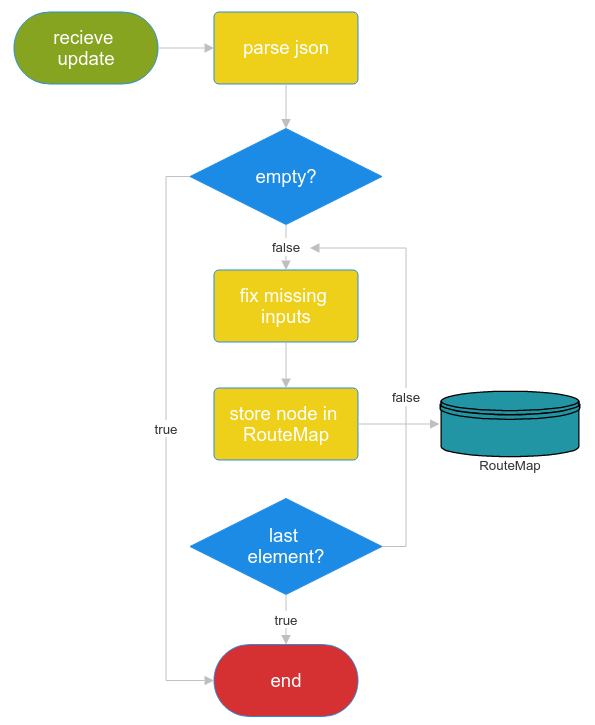
\includegraphics[width=0.8\textwidth]{nodegen-flow.png}
\end{center}
\fi
The router maps connections between extensions in a Redis database, allowing extensions to remain unaware of the destinations for their outputs. Using Python's Pickle library, the system enables the transmission of diverse data types, including 3D models and tensor arrays.

\subsection{FDTD Simulator}

Examples from Laportes\cite{laporte20} original library were tailored to specific scenarios. We extended these to be more versatile by introducing parameters for material properties, boundary conditions, and source configurations. Though this library claimed CUDA accelerated code, it would not work in any configuration tried during development. After communicating this to the original developer, and trying several bug-fixes and patches as well as utilizing input from a Language Model, we had simply run out of time to develop parallelized code in order to reach our original goals. Instead we settled on using PyTorch as the computation backend.

Post adaptation of the FDTD core, a user interface (UI) was developed to allow intuitive setup and execution of simulations. The UI was designed to be simple yet effective, enabling users to configure simulations easily and visualize results in real time. The UI offers real-time visualization of the simulation grid and allows the option between Matplotlib and Plotly for visualizations.
For common simulation setups, users can choose from pre-configured settings, which simplifies the simulation process and saves time.



%\subsubsection{MagiSimObject File Format}

%\begin{center}
%\begin{table}[h]
%	\begin{tabular}{|l|l|l|l|l|l|}
%		\hline
%		\rowcolor[HTML]{C0C0C0} 
%		\textbf{Name}                 & \textbf{Magic Number} & \textbf{Version} & \textbf{Name}                 & \textbf{N/A} & \textbf{Checksum}              \\ \hline
%		\cellcolor[HTML]{C0C0C0}Size  & 4*8                   & 4*8              & 32*8                          & 20*8         & 12*8                           \\ \hline
%		\cellcolor[HTML]{C0C0C0}Value & "MSOF"                & "1"              & \textless{}Name\textgreater{} & None         & \textless{}CRC32\textgreater{} \\ \hline
%	\end{tabular}
%\end{table}
%d\end{center}


\subsection{Software Distribution}
\textbf{It is certain that the importance of keeping scientific resources and research available to the public can not be stressed enough.}

Hence the source code of Magisim is distributed under the GNU Lesser General Public License (LGPLv3) allowing for all content within the non-commercial section of the codebase to be released publicly. The desicion to use LGPLv3 instead of GNU Public License v3 (GPLv3) was made in order to give third party developers more freedom to chose a license that fits their software, while being able to redistribute altered versions of our code.
GitHub was chosen for version management and publishing.


\newpage
\section{Result}
% images of the software UI?´
\subsection{User interface}


% outline the basic process of running a simulation
\subsection{Simulation Process}
Once the software is started using the included script, a user interface is available at \textit{http://localhost:8000}. By default, the program listens only for connections from the same computer, but this can be modified in the configuration file.

Our interface lands the user at the greeter, see figure \ref{fig:magisimgreeter}. From here, the user can browse through all installed extensions (represented as tabs, denoted workspaces) and perform actions.
To run a simple simulation, the connection between extensions must be formed by creating and saving a node graph, see figure \ref{fig:magisimnodegraph}. 

Once the connection has been formed, a model can be uploaded to the slicing interface (note that this is only necessary for simulating a 3d object represented in 2d space, 2d only simulations can be done by either generating a simple lens object or uploading a \textit{Magisim Object (.mso)} file), as seen in figure \ref{fig:magisimstl}. 

The user can then enter the \textit{MSEMS} workspace and edit the object parameters as well as configure sources, PML:s and detectors for analysis. (figure \ref{fig:msemsgridprep} and \ref{fig:msemsgridprops})

After configuring the crucial parameters, the user switches to the simulation sub-workspace, see figure \ref{fig:msemssim}. Here the user chooses how many timesteps will be simulated and if detector readings should be generated.

Once the simulation is complete, a resulting image can be saved using the plot viewer interface.


% describe the process of installing extensions using the extension manager

\subsection{Simulation Performance Characterization}
% showcase statistics, speeds and simulation images
A benchmarking simulation was set up, with an initial grid size of $250^{2}$, where each unit represents $\frac{1}{10}\lambda$. A lens object was subsequently added to the grid. A point source was placed at $(15,20)$ configured as a continuous wave function with the wavelength of 635nm.
\begin{center}
	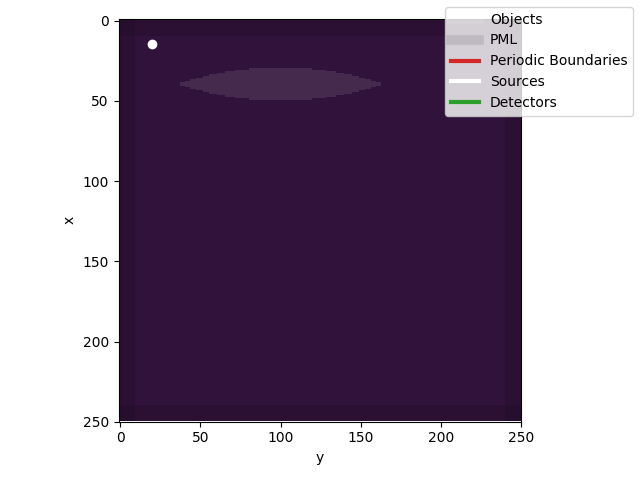
\includegraphics[width=0.8\textwidth]{gridplan.png}
\end{center}
Five simulations were ran in conjunction with a timer function and the result was appended to a spreadsheet (see figure \ref{fig:benchmarkdata}). This process was then repeated two more times, each with a quadrupled grid size.



\begin{center}
	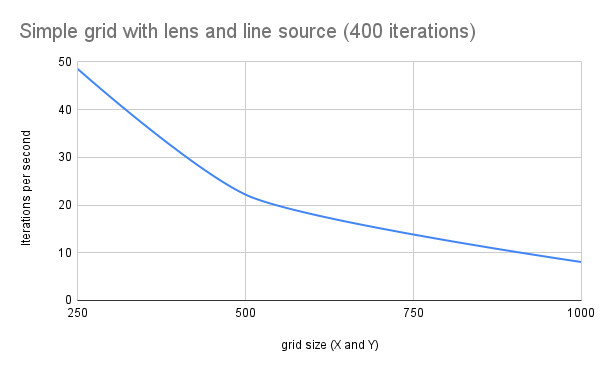
\includegraphics[width=0.8\textwidth]{gridstats.png}
\end{center}
When the simulation grid size quadruples, resulting in a fourfold increase in the space (\( n \) becomes \( 4n \)), the calculation speed drops by 50\%. This change can be represented by the equation:

\[
S' = \frac{1}{2} S
\]

From this, we infer that speed \( S \) is inversely proportional to the square root of the simulation space size \( n \):

\[
S(n) \propto \frac{1}{\sqrt{n}}
\]

This relationship shows that the computation speed scales as \( O(n^{-1/2}) \) in big-O notation, which is significantly worse than initially planned. This is most likely due to our plotting code, since it has to convert the simulation grid points into a plot every single frame, in order to get real time simulations. This could be solved by animating the simulation and then pushing the result to the front-end. This would however add significant loading times and would degrade user experience drastically. Another potential source of performance decreases lie within the simulation code itself as the simulation is inherently multidimensional. Currently, the calculations are performed serially using the CPU, accellerating the code using i.e. Nvidia CUDA technology would reduce the processing time. With parallelization, the effectiveness of a multidimensional computation can be increased drastically, essentially allowing for $n-1$ dimensional computation as illustrated in figure \ref{fig:serialsim} and \ref{fig:parsim}.




\newpage
\section{Conclusion}
% We sucessfully wrote a modular interface for simulations, with a functional node graph interface for data flow programming aw well as a working extension system

% We sucessfully integrated FDTD simulation code as a extension.

% Lacking team effort led to less productivity

% Out of date non-commercial code without support led to compromises in speed

% Lackluster CUDA Acceleration support due to aforementioned abandoned code

% AI code quality and limited context windows of currently available language models led to weak code quality that needed to be thoroughly checked before use

% Recent rapid increase of open source software, like in the early 2000s after the IT boom, potentially in connection with layoffs.

The development of Magisim aimed to provide a modular and accessible tool for electromagnetic simulation, with specific emphasis on educational use and ease of expansion. This conclusion outlines the major achievements and reflects on the challenges faced throughout the project.

\textbf{Achievements:}
\begin{itemize}
	\item \textbf{Modular Interface:} A significant achievement of this project was the creation of a modular interface featuring a functional node graph interface for data flow programming. This interface supports dynamic interaction with the simulation processes and enhances user experience by providing intuitive control over complex simulations.
	\item \textbf{FDTD Simulation Integration:} Successfully integrating the Finite-Difference Time-Domain (FDTD) simulation code into the system as an extension. This integration underscores the interface’s capacity to handle advanced computational models and adapt to diverse simulation requirements.
	\item \textbf{User Interface Development:} The selection and implementation of Gradio as the UI framework facilitated rapid prototyping and effective user interaction, which has been pivotal in making the simulation tool more accessible to non-experts.
\end{itemize}

\textbf{Challenges:}
\begin{itemize}
	\item \textbf{Team Collaboration:} The project faced hurdles in team coordination, impacting productivity. Enhancing communication, project management practices and increasing group motivation could mitigate similar issues in future developments.
	\item \textbf{Outdated and Unsupported Code:} Dependency on out-of-date, unsupported code led to significant setbacks. Future efforts will need to focus on either updating this code or replacing it with more current, supported alternatives.
	\item \textbf{Limited CUDA Acceleration:} The lack of effective CUDA acceleration due to the outdated codebase was a significant technical challenge, which limited the performance enhancements expected from such technologies.
	\item \textbf{ML Assistance Limitations:} Utilizing Machine Learning Models to assist in code generation presented challenges, particularly in maintaining high code quality. This aspect underscores the necessity for thorough validation and refinement of LLM-generated code before its integration into production environments.
\end{itemize}

\newpage
\addcontentsline{toc}{section}{References} 
\printbibliography

\newpage
\appendix
\appendixpage
\addappheadtotoc

\begin{figure}[h]
	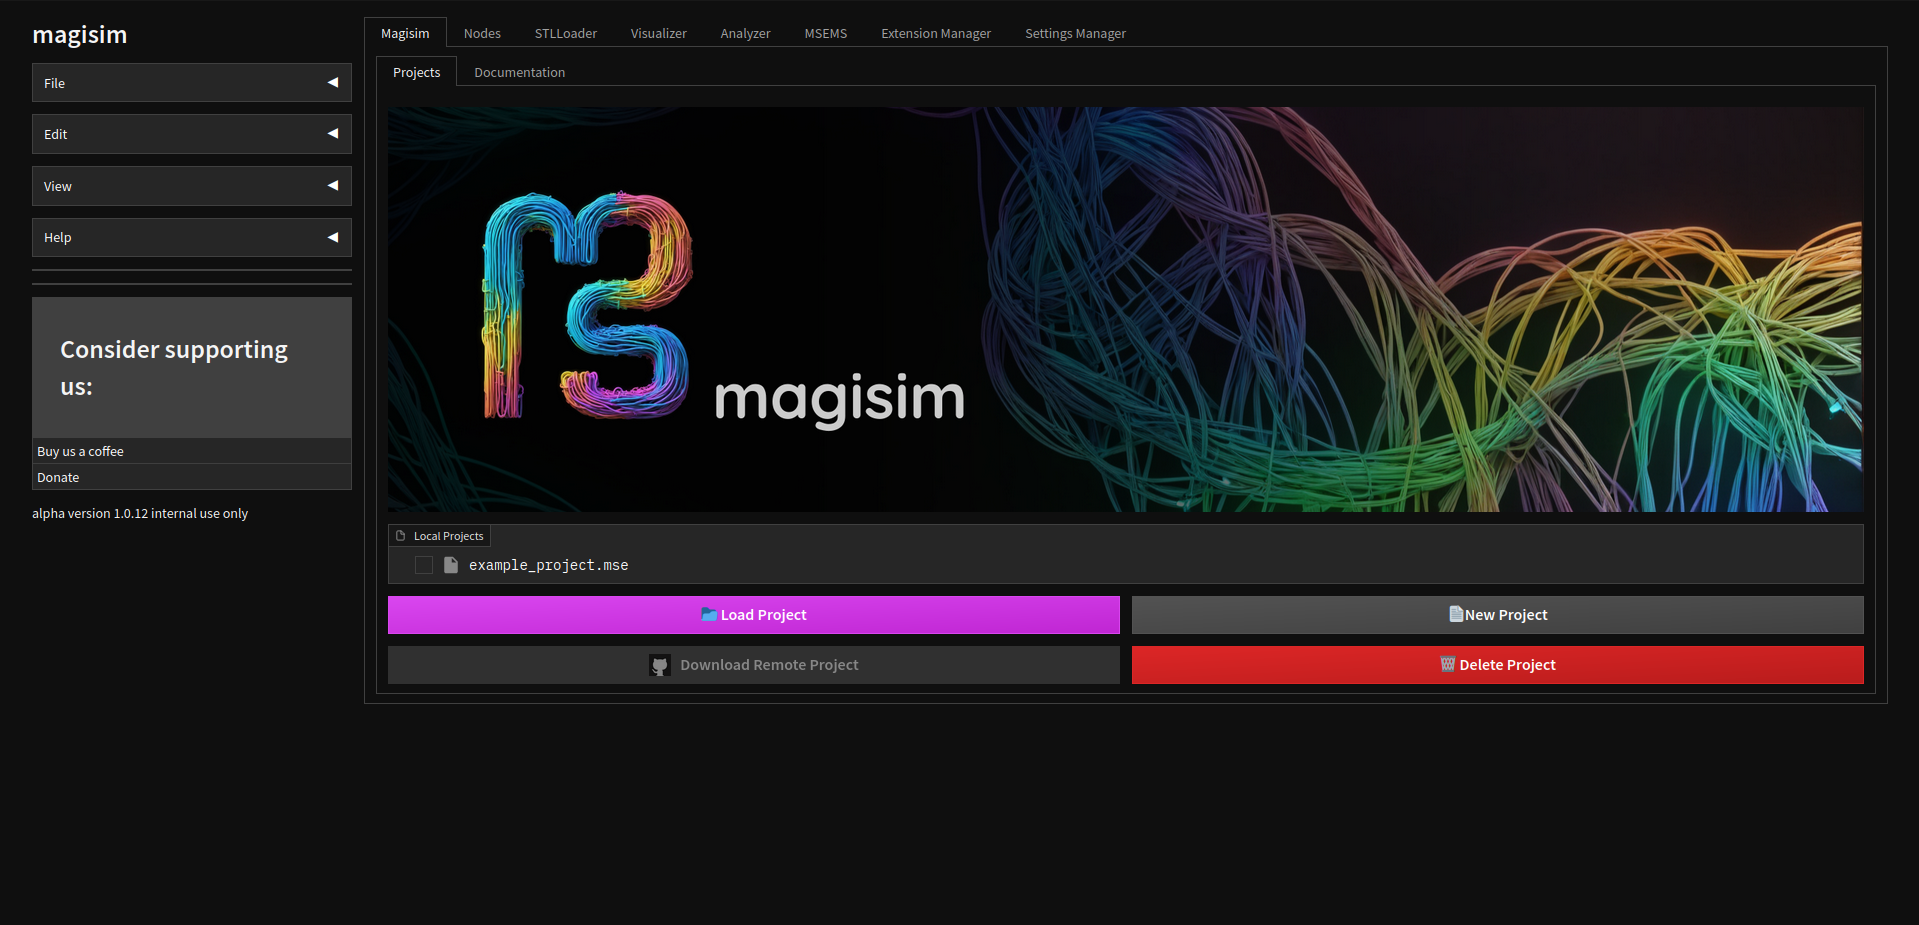
\includegraphics[width=\textwidth]{magisim-screenshot-0001.png}
	\caption{Magisim Greeter}
	\label{fig:magisimgreeter}
\end{figure}
\begin{figure}[h]
	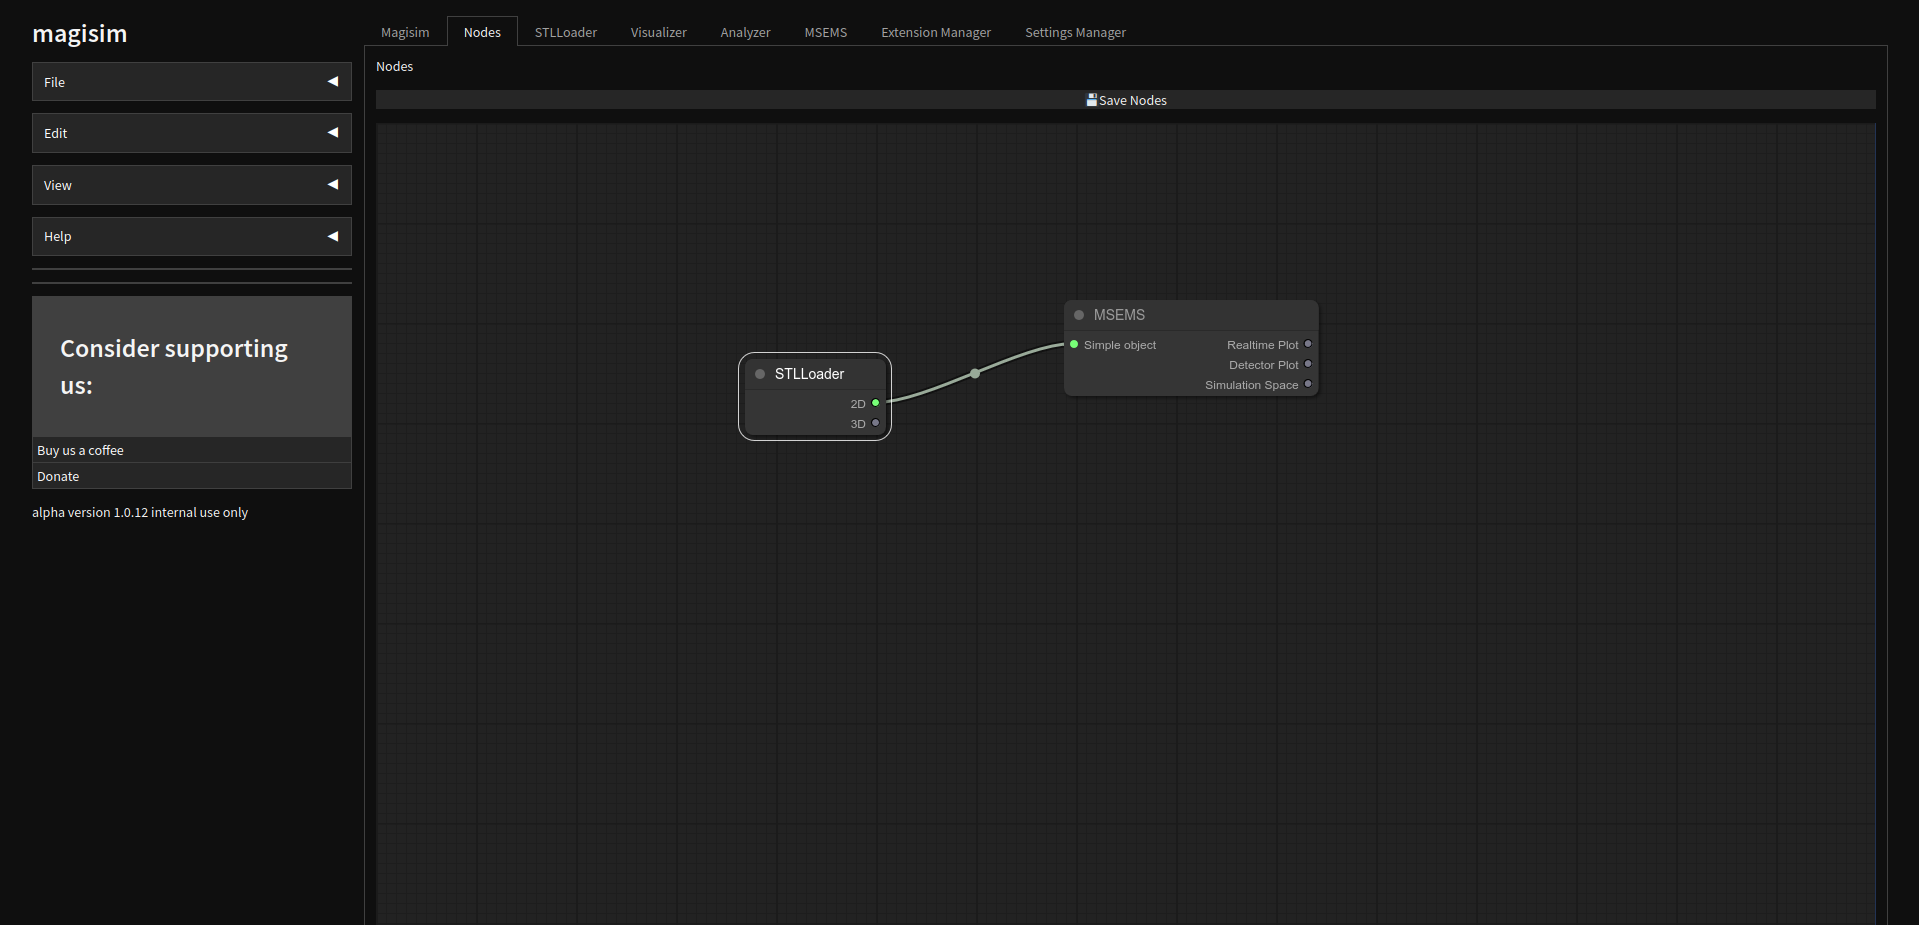
\includegraphics[width=\textwidth]{magisim-screenshot-0002.png}
	\caption{Magisim Node Graph Interface}
	\label{fig:magisimnodegraph}
\end{figure}
\newpage
\begin{figure}[h]
	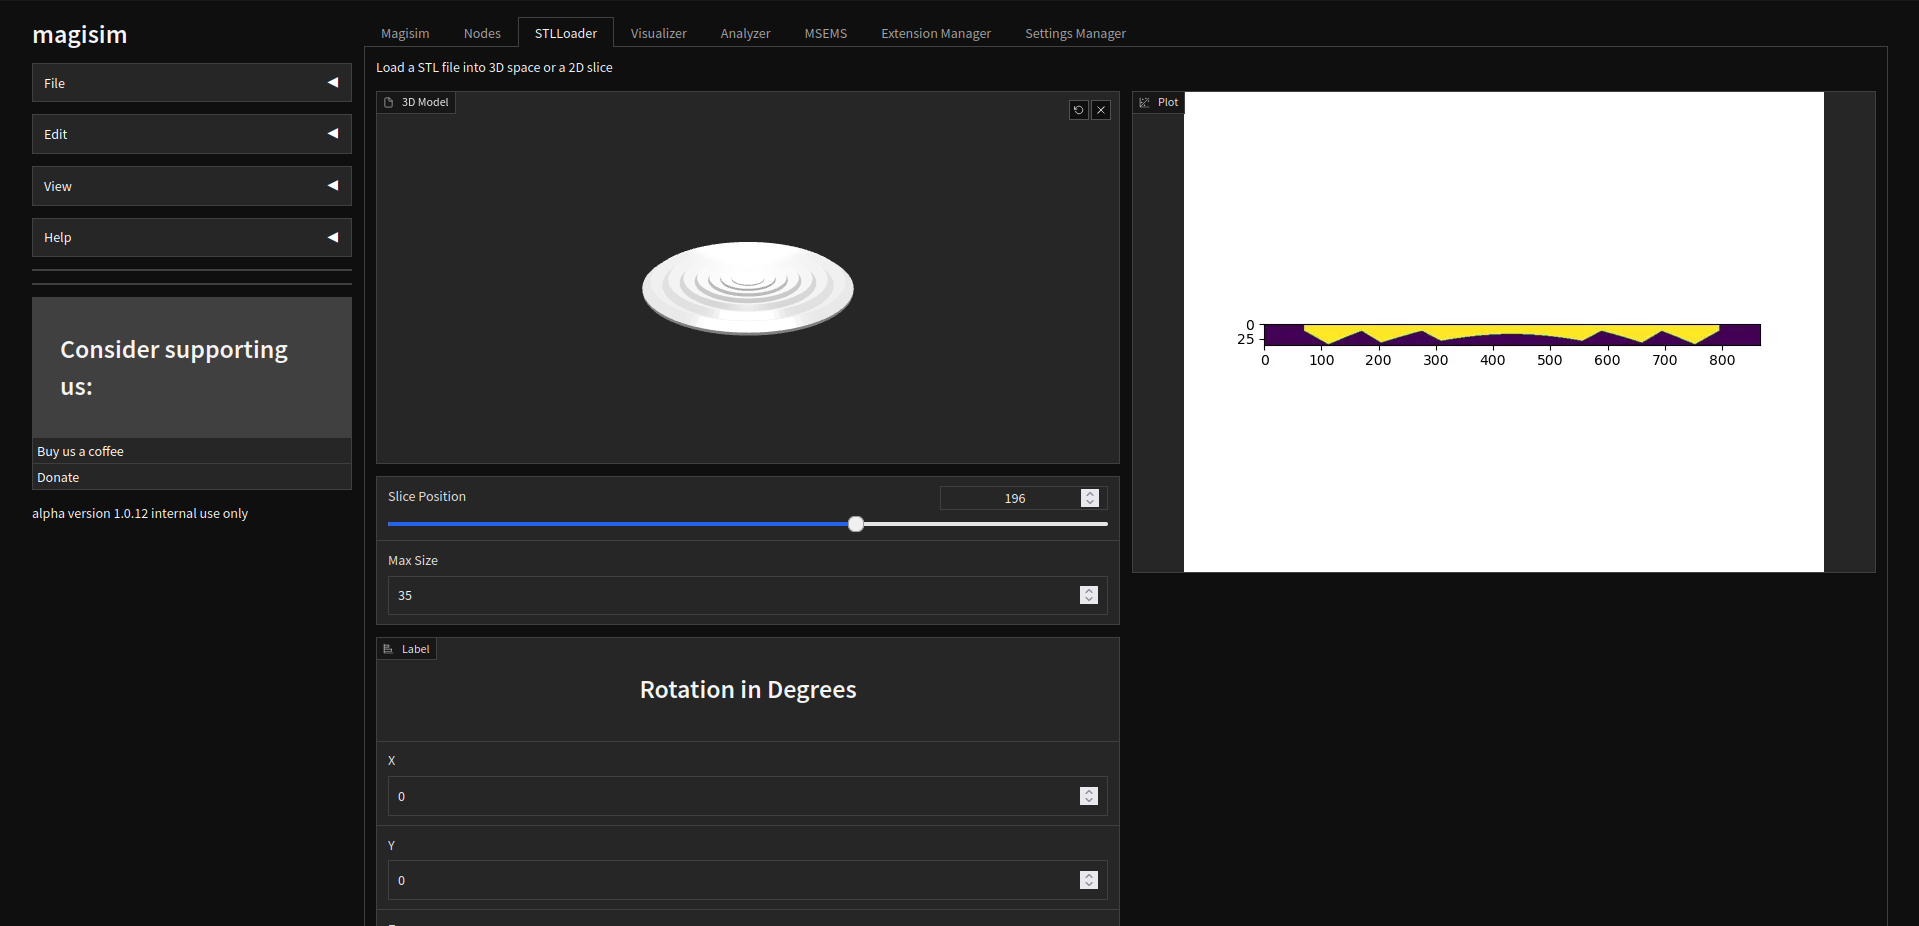
\includegraphics[width=\textwidth]{magisim-screenshot-0003.png}
	\caption{Magisim 3D Slicer}
	\label{fig:magisimstl}
\end{figure}
\begin{figure}[h]
	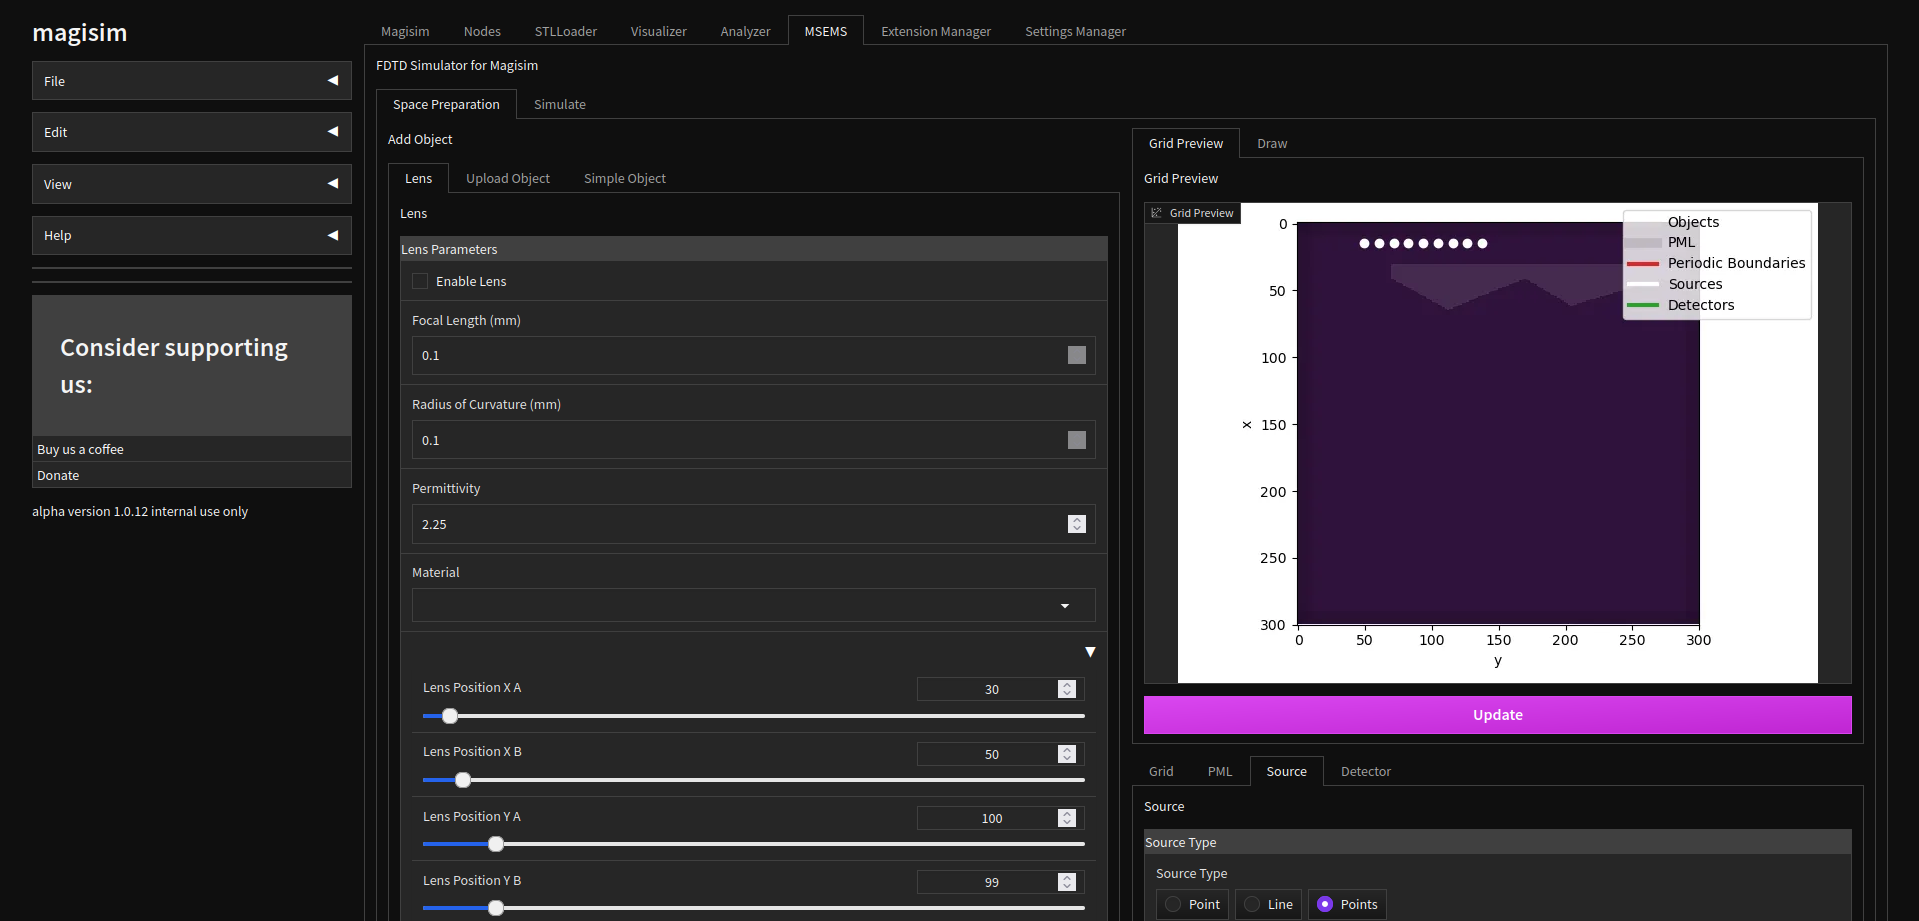
\includegraphics[width=\textwidth]{magisim-screenshot-0005.png}
	\caption{MSEMS Grid Preparation Interface}
	\label{fig:msemsgridprep}
\end{figure}
\newpage
\begin{figure}[h]
	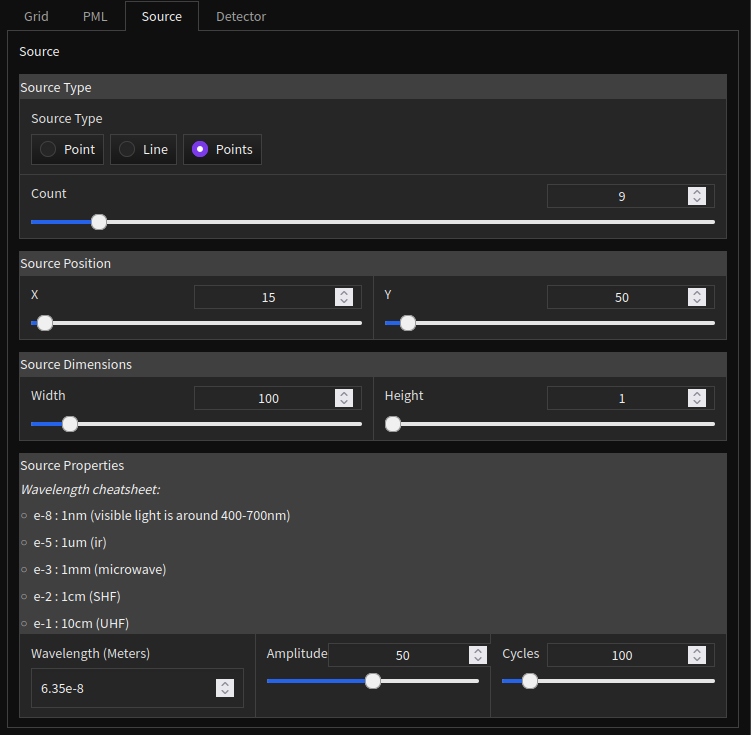
\includegraphics[width=\textwidth]{magisim-screenshot-0006.png}
	\caption{MSEMS Source Properties}
	\label{fig:msemsgridprops}
\end{figure}
\newpage
\begin{figure}[h]
	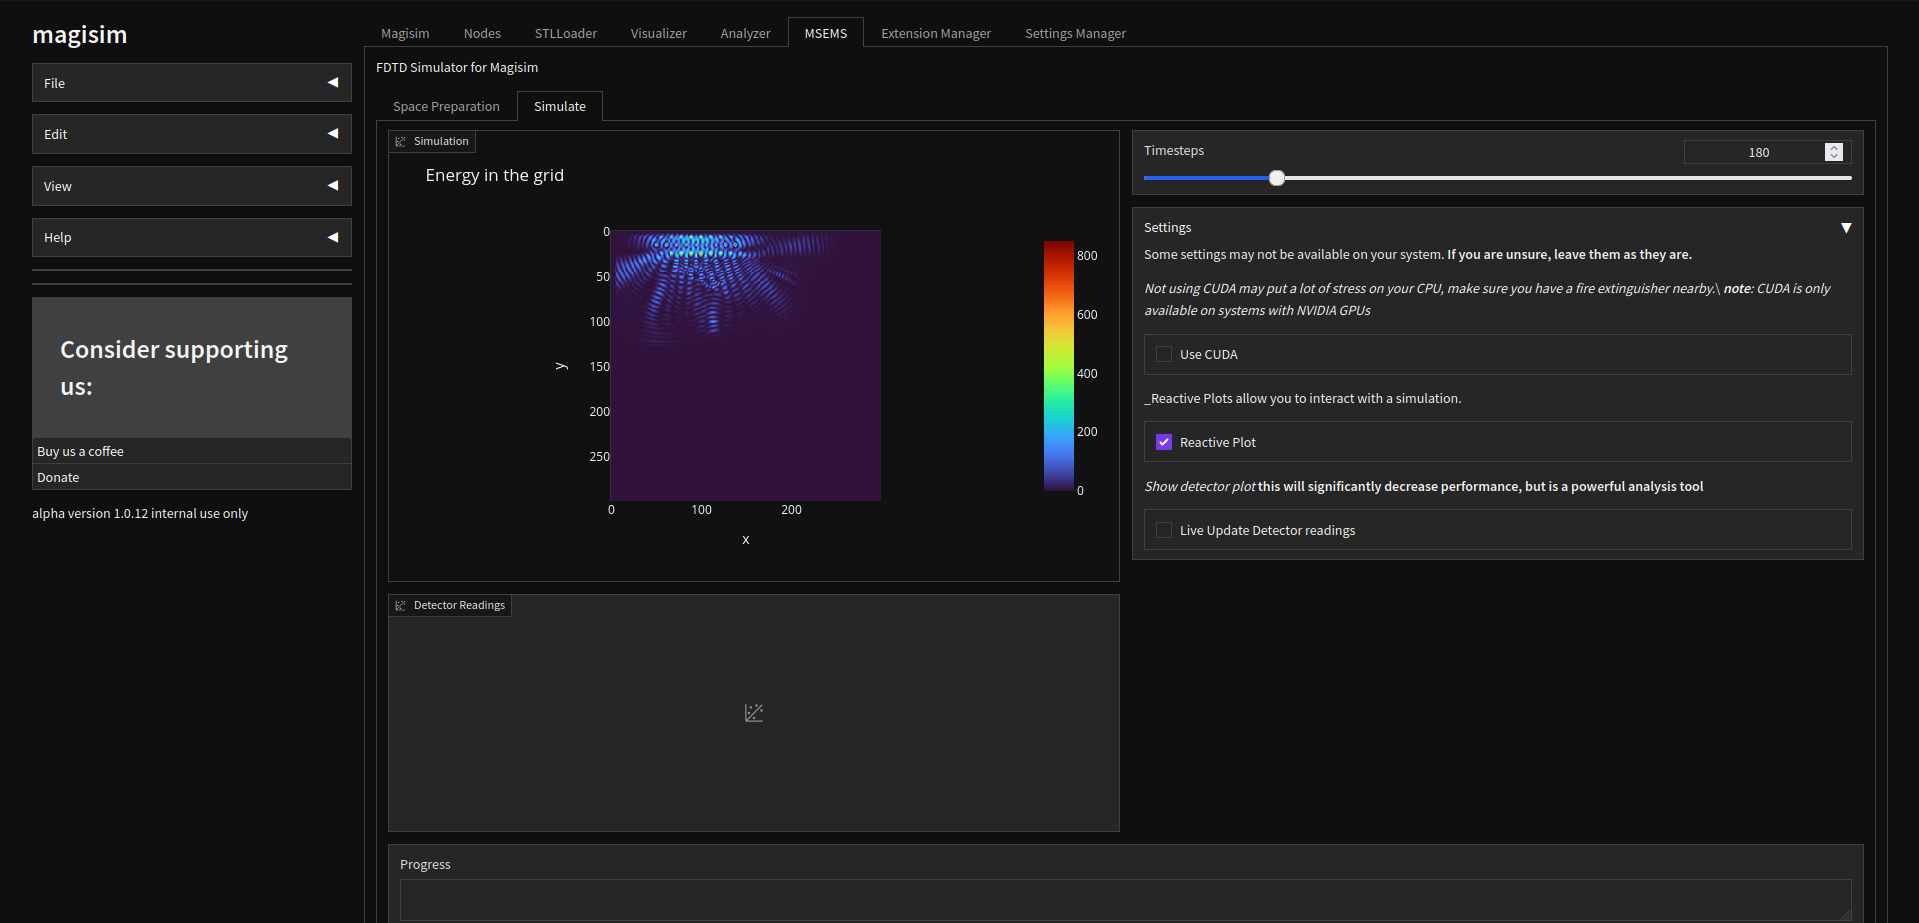
\includegraphics[width=\textwidth]{magisim-screenshot-0007.png}
	\caption{MSEMS Simulation}
	\label{fig:msemssim}
\end{figure}
\begin{center}
\begin{figure}[h!]
	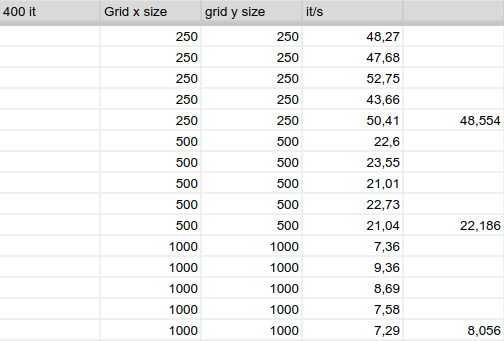
\includegraphics[width=0.8\textwidth]{benchmarkdata.png}
	\caption{Benchmarking Data}
	\label{fig:benchmarkdata}
\end{figure}
\end{center}
\newpage
\begin{figure}[h]
	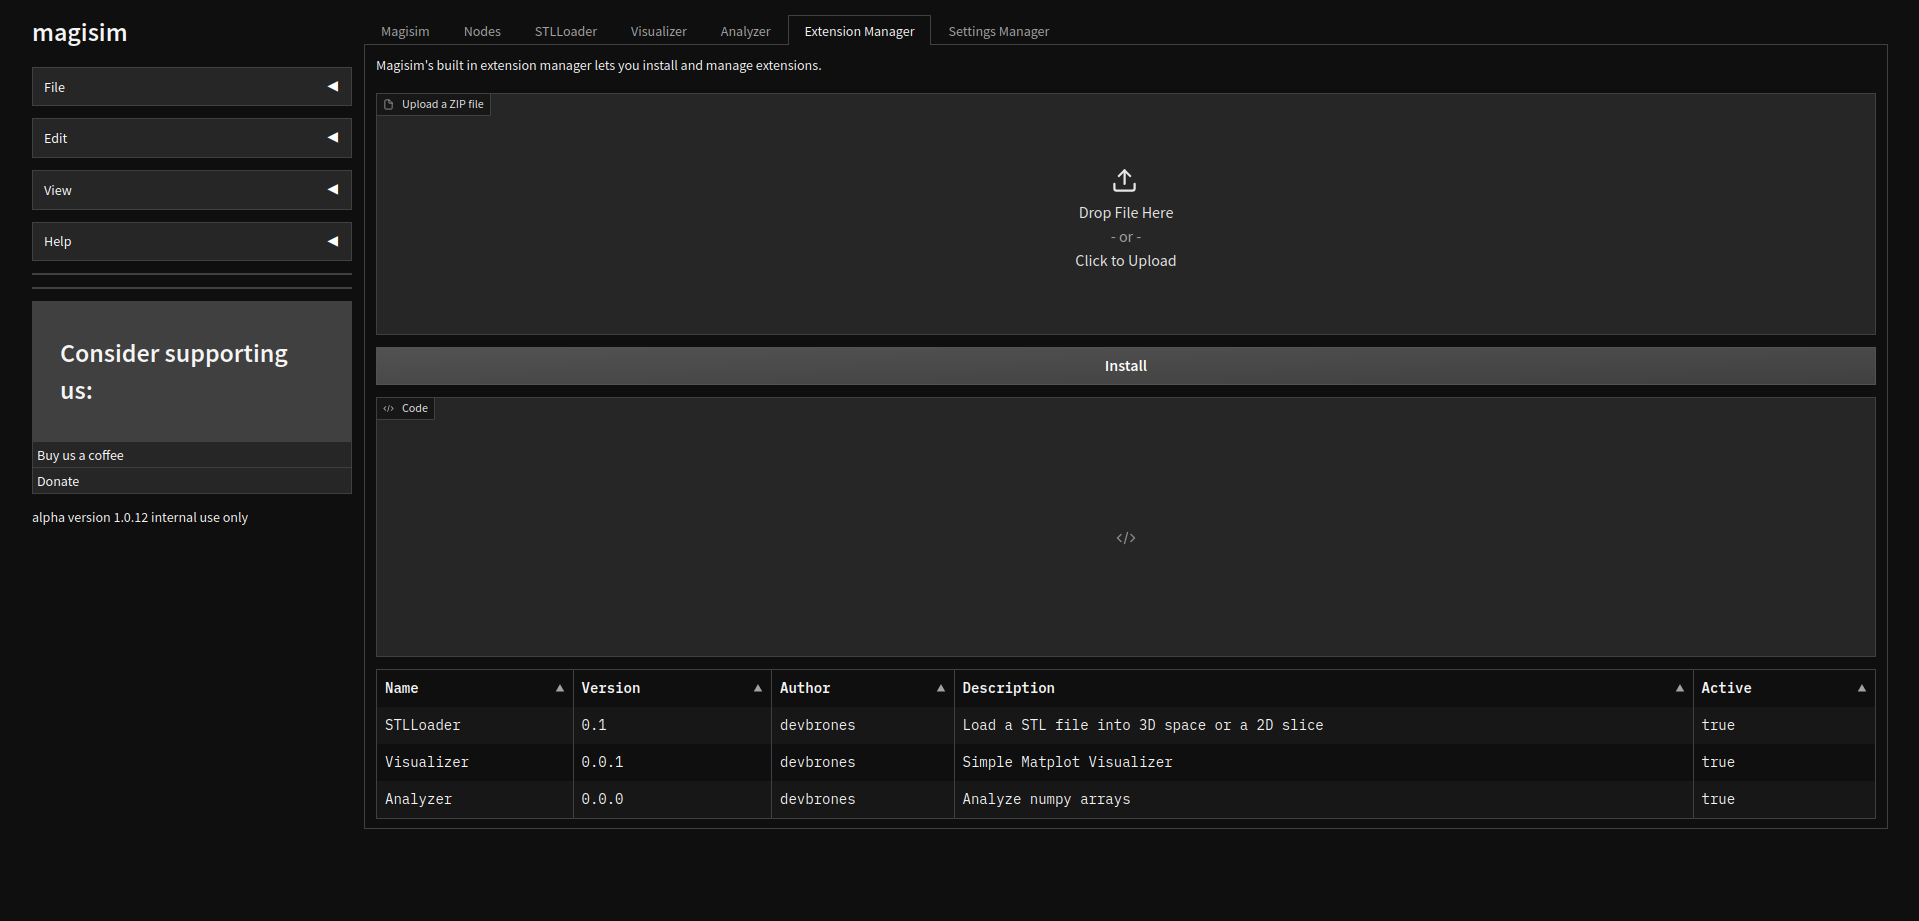
\includegraphics[width=\textwidth]{magisim-screenshot-0008.png}
	\caption{Extension Manager}
	\label{fig:exmgr}
\end{figure}
\begin{figure}[h]
	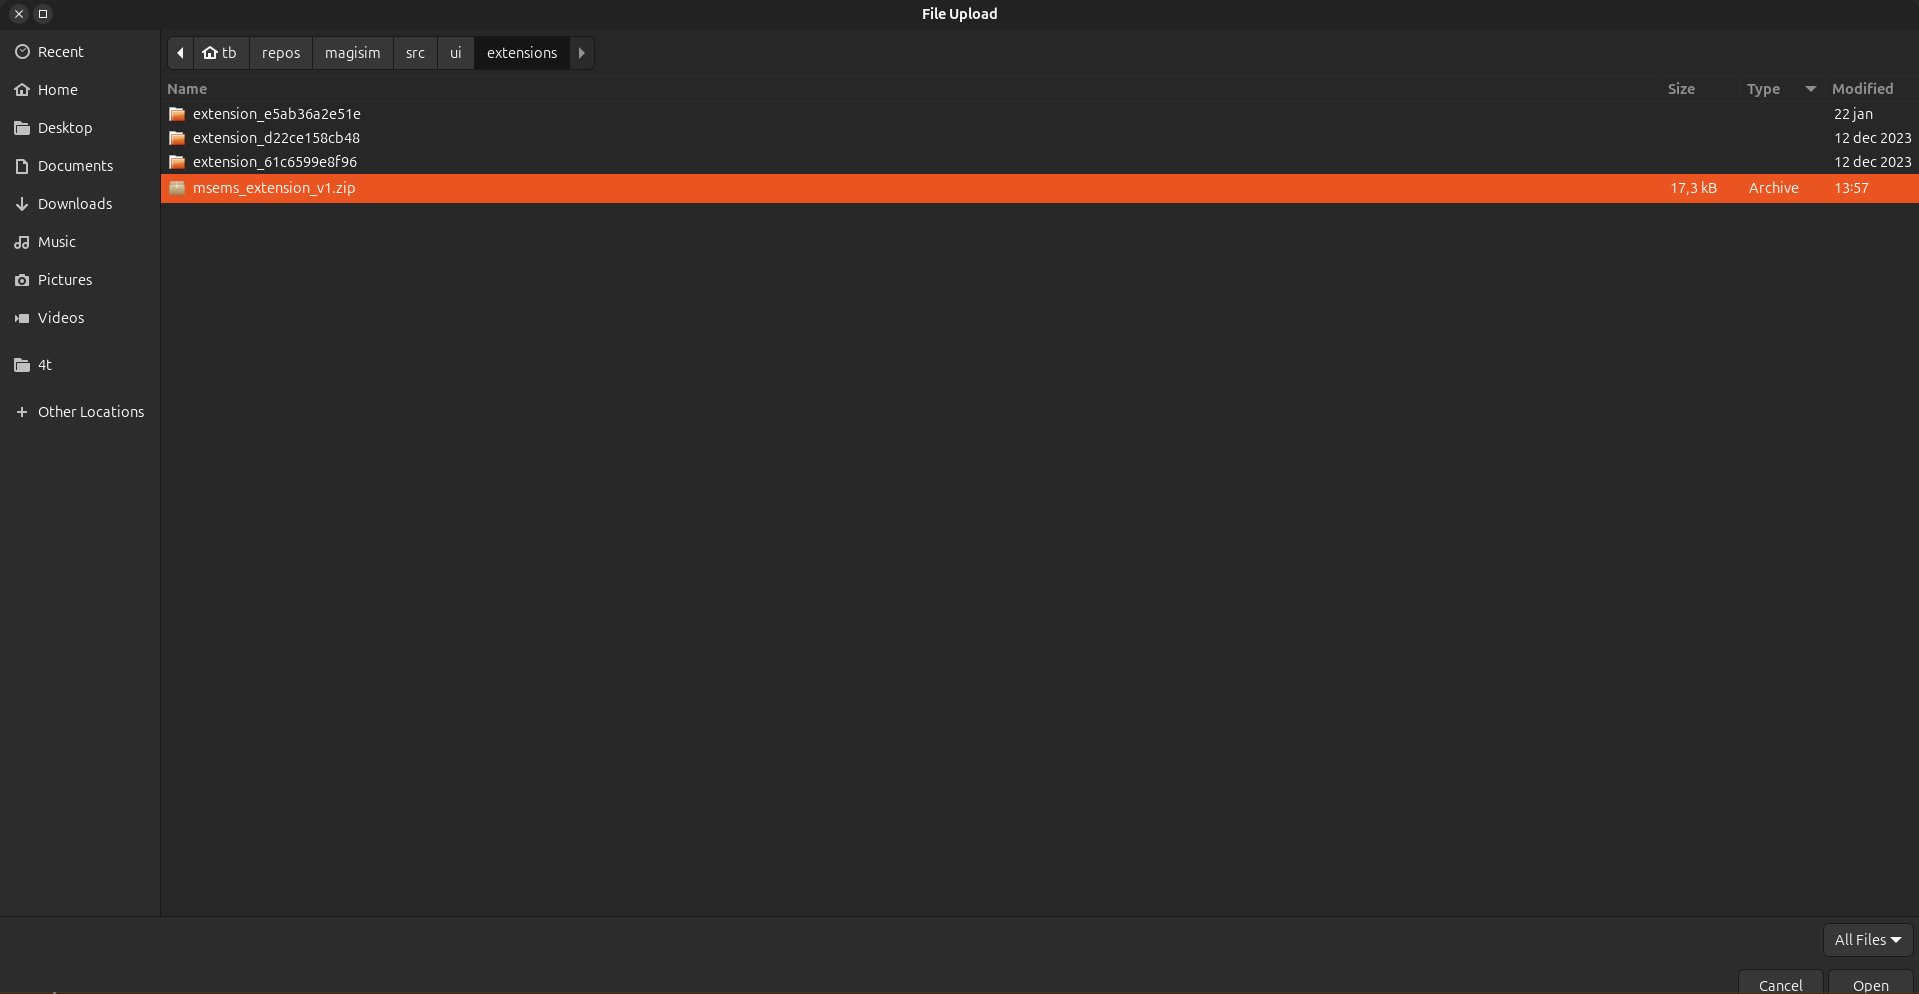
\includegraphics[width=\textwidth]{magisim-screenshot-0009.png}
	\caption{Selecting a extension zip file}
	\label{fig:selexzip}
\end{figure}
\newpage
\begin{figure}[h]
	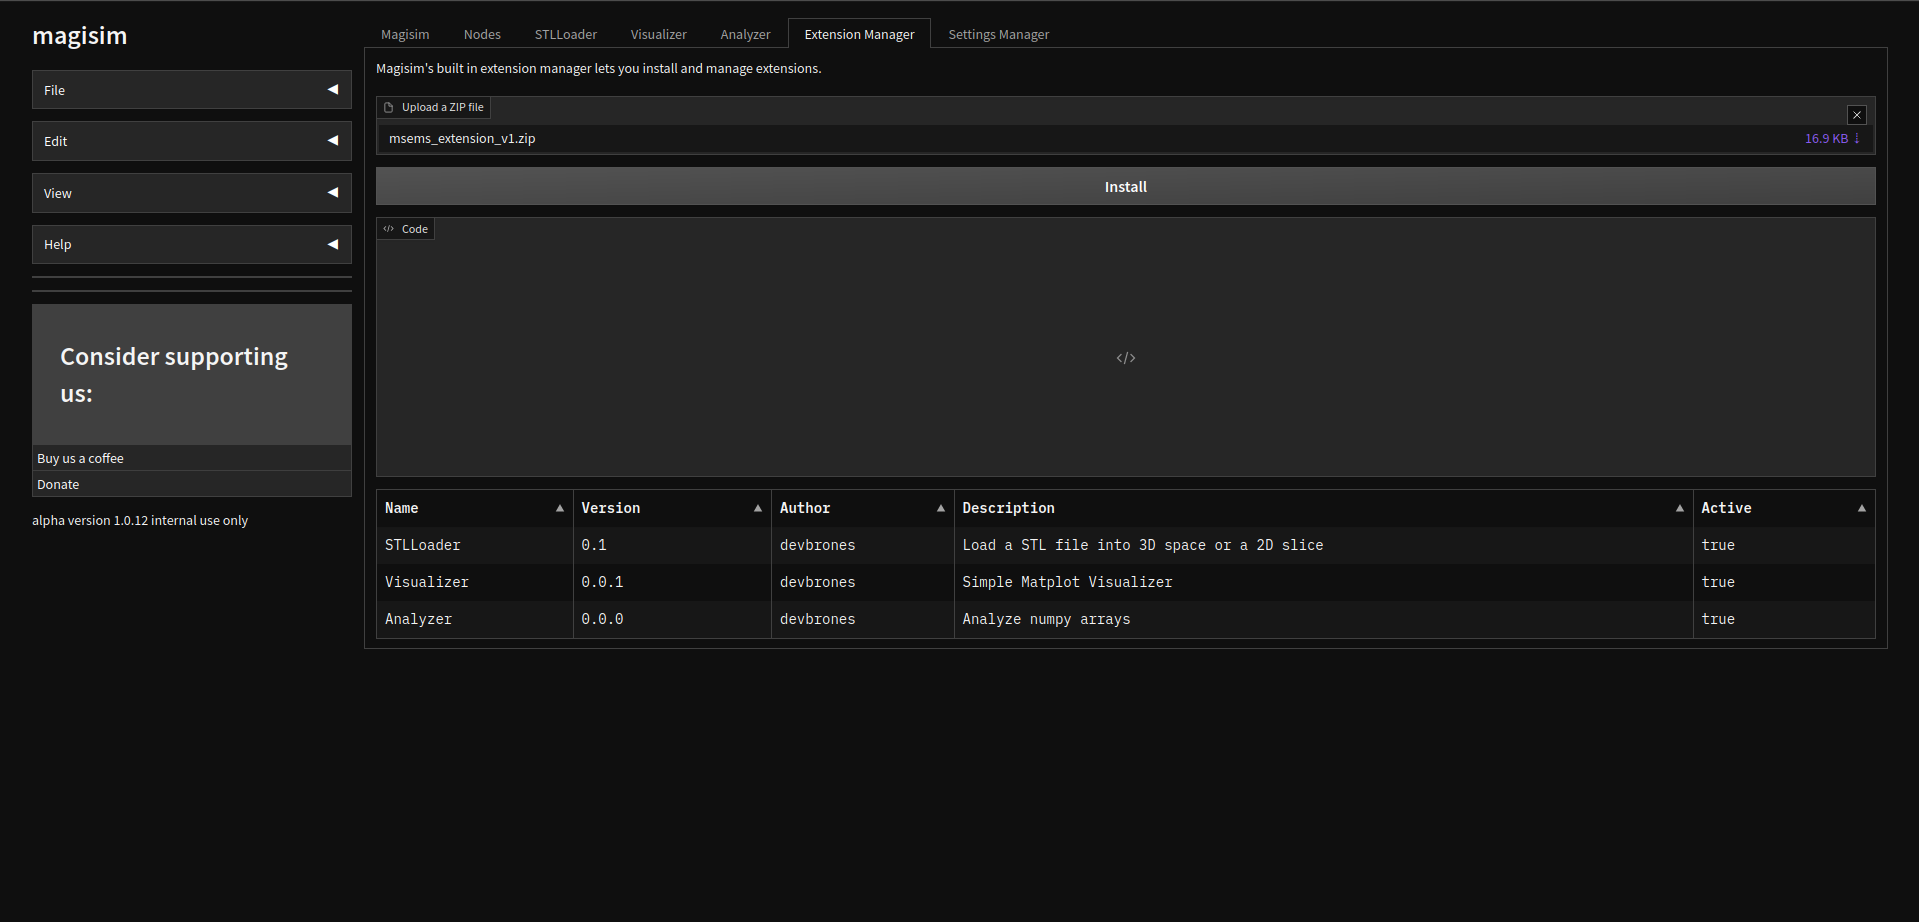
\includegraphics[width=\textwidth]{magisim-screenshot-0010.png}
	\caption{Extension uploaded to Magisim}
	\label{fig:exuplsucc}
\end{figure}
\begin{figure}[h]
	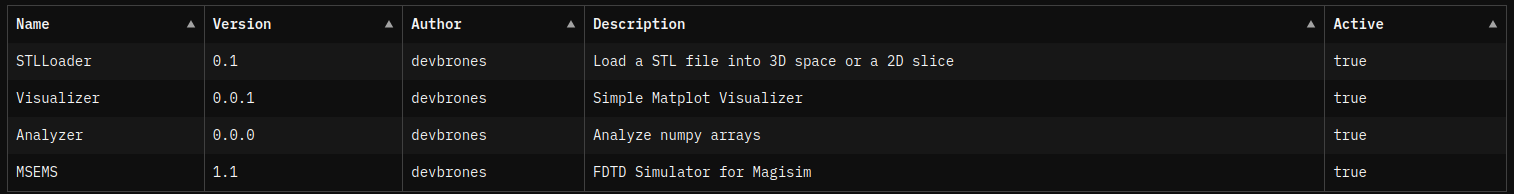
\includegraphics[width=\textwidth]{magisim-screenshot-0011.png}
	\caption{Extension installed after restart}
	\label{fig:exvisreb}
\end{figure}
\begin{figure}[h]
	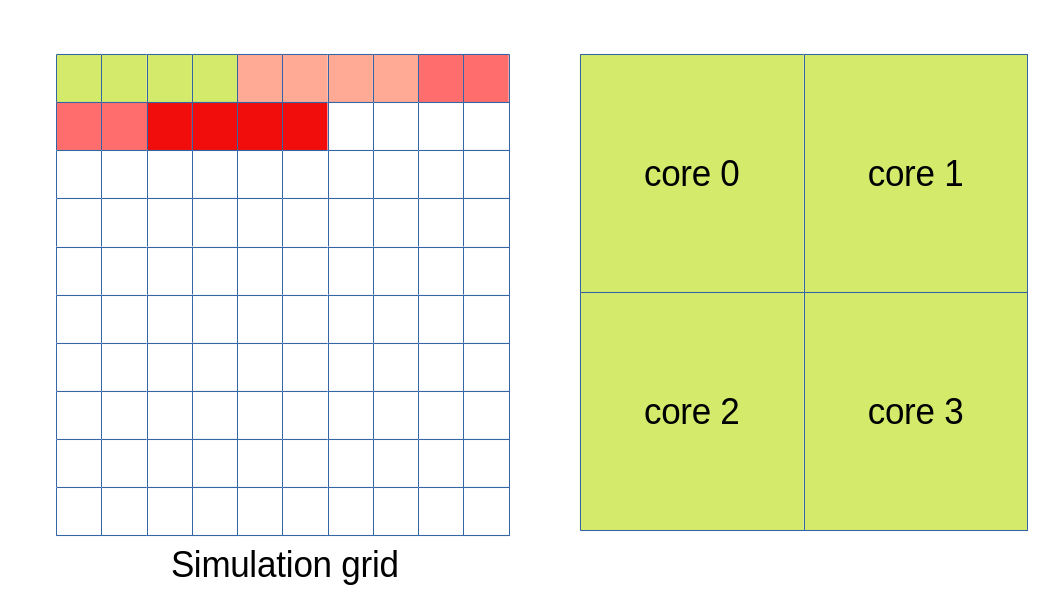
\includegraphics[width=\textwidth]{simserial.png}
	\caption{Serial Computation on a quad core CPU, red indicates next segment}
	\label{fig:serialsim}
\end{figure}
\begin{figure}[h]
	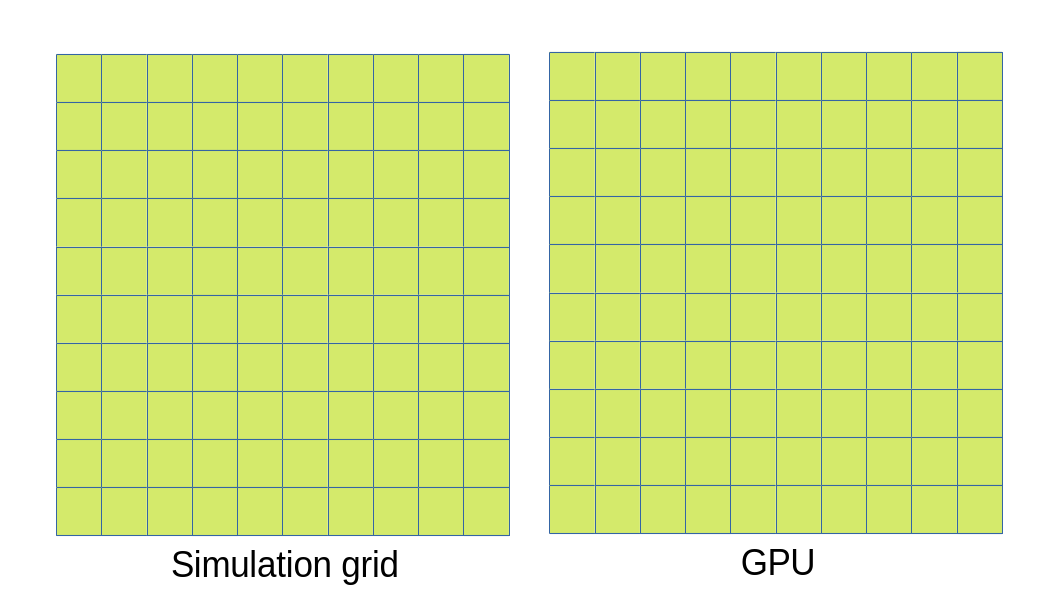
\includegraphics[width=\textwidth]{simpar.png}
	\caption{Parallel Computation on a n-Core GPU, simultaneous cell processing}
	\label{fig:parsim}
\end{figure}



\begin{center}
	\large\textbf{Written in \LaTeX}
\end{center}



\end{document}          
